\documentclass{beamer}


\usepackage[utf8]{inputenc}
\usepackage{amsmath}
\usepackage{amsfonts}
\usepackage{amssymb}
\usepackage{graphicx}
\usepackage{ragged2e}  % `\justifying` text
\usepackage{booktabs}  % Tables
\usepackage{tabularx}
\usepackage{tikz}      % Diagrams
\usetikzlibrary{calc, shapes, backgrounds}
\usepackage{amsmath}
\usepackage{amssymb}
\usepackage{dsfont}
\usepackage{url}       % `\url
\usepackage{listings}  % Code listings
\usepackage[T1]{fontenc}
\usepackage[percent]{overpic}
\usetikzlibrary{trees}
\usepackage[absolute,overlay]{textpos}

\usepackage{theme/beamerthemehbrs}

\author[MAS]{Author: Hassan Umari \\ Edited by Vamsi Krishna \& Hamsa Datta}

\title{Introduction to Robot Operating System (ROS)}
\subtitle{Foundation course}
\institute[HBRS]{Hochschule Bonn-Rhein-Sieg}
\date{\today}
\subject{ROS2 workshop}

% \thirdpartylogo{path/to/your/image}


\begin{document}
{
\begin{frame}
\titlepage
\end{frame}
}

%---------------------------

\section{Scenario}

\begin{frame}{Scenario}
    \centering
    \begin{overpic}[width=.3\linewidth]{figures/analogy3.png}
        \put (2,102) {Mapping algorithm}
        \put (24,74) {s/w} 
        \put (11,49) {Laser driver} 
        \put (-25,10) {Laser scanner} 
    \end{overpic}
\end{frame}


\begin{frame}{Scenario}
    \begin{overpic}[width=.8\linewidth]{figures/analogy4.png}
        \put (34,72) {Mapping algorithm}
        \put (48,54) {s/w}
        \put (2.3,29) {Laser driver}
        \put (38,29) {Laser driver}
        \put (75,29) {Laser driver}
    \end{overpic}
\end{frame}

\begin{frame}{Scenario}
    \begin{overpic}[width=.8\linewidth]{figures/analogy5.png}
        \put (34,72) {Mapping algorithm}
        \put (46.5,54) {ROS}
        \put (2.3,29) {Laser driver}
        \put (38,29) {Laser driver}
        \put (75,29) {Laser driver}
        \put (105,10) {\footnotesize Different hardware}
    \end{overpic}
\end{frame}

\begin{frame}{Scenario}
    \begin{overpic}[width=.8\linewidth]{figures/analogy6.png}
        \put (34,72) {Mapping algorithm}
        \put (46.5,54) {ROS}
        \put (2.3,29) {Laser driver}
        \put (38,29) {Laser driver}
        \put (75,29) {Laser driver}
        \put (105,10) {\footnotesize Different hardware}
        \put (105,30) {\footnotesize Different drivers}
    \end{overpic}
\end{frame}

\begin{frame}{Scenario}
    \begin{overpic}[width=.8\linewidth]{figures/analogy7.png}
        \put (34,72) {Mapping algorithm}
        \put (46.5,54) {ROS}
        \put (2.3,29) {Laser driver}
        \put (38,29) {Laser driver}
        \put (75,29) {Laser driver}
        \put (105,10) {\footnotesize Different hardware}
        \put (105,30) {\footnotesize Different drivers}        
        \put (105,58) {\footnotesize Data received in}
        \put (105,54) {\footnotesize the same message}
        \put (105,50) {\footnotesize format}
    \end{overpic}
\end{frame}

\begin{frame}{Scenario}
    \begin{overpic}[width=.8\linewidth]{figures/analogy7.png}
        \put (34,72) {Mapping algorithm}
        \put (46.5,54) {ROS}
        \put (2.3,29) {Laser driver}
        \put (38,29) {Laser driver}
        \put (75,29) {Laser driver}
        \put (105,10) {\footnotesize Different hardware}
        \put (105,30) {\footnotesize Different drivers}        
        \put (105,58) {\footnotesize Data received in}
        \put (105,54) {\footnotesize the same message}
        \put (105,50) {\footnotesize format}
        \put (105,72) {\footnotesize No change}
    \end{overpic}
\end{frame}

\begin{frame}[plain]{}
    \centering
    \includegraphics[width=.66\linewidth]{figures/stop_reinventing_theWheel.jpg}
    
\tiny{http://www.willowgarage.com/blog/2010/04/27/reinventing-wheel}
\end{frame}


\section{What is ROS?}

\subsection{What ROS is}
\begin{frame}{What ROS is}

    \begin{itemize}
        \item Short for: Robot Operating System.
        \item A collection of libraries and tools.
        \item It helps software developers create robot
        applications. 
    \end{itemize}
\end{frame}

\begin{frame}{What ROS is}

    \begin{itemize}
        \item A way to standardize writing software for robots.
        \item It enhances {\huge code reusability} \includegraphics[scale=0.02]{figures/recycling.png}.
        \item ROS is open-source \includegraphics[scale=0.09]{figures/open_source.png}.
        \item It is a meta-operating system.
        \item ROS is installed on top of Linux/ Windows/ Mac.

    \end{itemize}
    
    % Meta operating system - is built on top of the operating system and allows different processes (nodes) to communicate with each other at runtime. It provides the services you would expect from an operating system, including hardware abstraction, low-level device control, implementation of commonly-used functionality, message-passing between processes, and package management. It also provides tools and libraries for obtaining, building, writing, and running code acROS2s multiple computers.
\end{frame}


\subsection{What ROS is NOT}
\begin{frame}{What ROS is NOT}
    \framesubtitle{Robot Operating System}
    \begin{itemize}
        \item It is NOT a programming language.
        \item It is NOT an integrated development environment
        (IDE).
        \item It is NOT a stand-alone operating system.
    \end{itemize}
\end{frame}


\subsection{Analogy between ROS and operating systems}

\begin{frame}{Analogy between ROS and operating systems}
    \begin{overpic}[width=.45\linewidth]{figures/analogy1.png}
        \put (130,80) {Software applications}
        \put (130,50) {work on}
        \put (130,20) {Different hardware}        
    \end{overpic}
\end{frame}

\begin{frame}{Analogy between ROS and operating systems}
    \begin{overpic}[width=.45\linewidth]{figures/analogy8.png}
        \put (130,77) {Robot applications}
        \put (3,75) {\scriptsize Mapping}
        \put (33,75) {\scriptsize Navigation}
        \put (66,75) {\scriptsize Pick \& place}
        \put (130,50) {work on}
        \put (130,20) {Different hardware}        
    \end{overpic}
\end{frame}




\begin{frame}[label=figs2]{Analogy between ROS and operating systems}
\centering
 \scalebox{0.9}{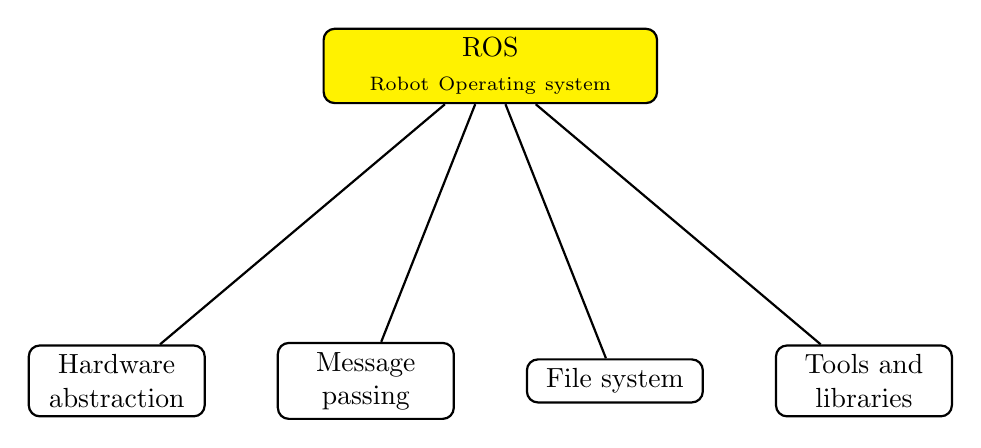
\begin{tikzpicture}[sibling distance=9em, level distance = 4.0cm, thick,
every node/.style = {shape=rectangle, rounded corners,
    draw, align=center}]]
\node [text width=4cm, fill = yellow]{ROS \\ \scriptsize Robot Operating system}
child { node [text width=2cm]{Hardware abstraction} }
child { node [text width=2cm]{Message passing} }
child { node [text width=2cm]{File system} }
child { node [text width=2cm]{Tools and libraries} };
\end{tikzpicture}}
\end{frame}


%---------------------------

\section{Features of ROS}

\begin{frame}{Features of ROS}

\begin{itemize}
        \item Language independent
        \item Distributed and modular
        \item A lot of libraries and tools
        \item Open source
        \item Active community
\end{itemize}
\end{frame}

\subsection{Language independent}

\begin{frame}{Language independent}
    \framesubtitle{Features of ROS}    
    \begin{itemize}
        \item ROS functionalities are implemented as a library in different programming languages (Python, C++, ...).
        \item  These libraries are referred to as ROS client libraries.
    \end{itemize}
\end{frame}

\begin{frame}{Language independent}
    \framesubtitle{Features of ROS}    
 
    ROS client libraries 

    \vspace{0.5cm}
    \centering
\scalebox{0.8}{%
  \begin{minipage}{\textwidth}
    \begin{itemize}
        \item ROS Supported Client libraries:
        \begin{itemize}
            \item Cpp, Python
        \end{itemize}
        \item ROS Community-maintained client libraries:
        \begin{itemize}
            \item C (micro-ROS) \hspace{7cm} 
            \item Java and Android \hspace{7cm} 
            \item Node.js \hspace{7cm}
            \item Rust
        \end{itemize}
        \item ROS support on MATLAB:
        \begin{itemize}
            \item Robotics System Toolbox \hspace{4.3cm} 
        \end{itemize}
    \end{itemize}
\end{minipage}%
}

% ROS2lisp - supports LISP - family of programming languages originally specified in 1958. As one of the earliest programming languages, Lisp pioneered many ideas in computer science, including tree data structures, automatic storage management, dynamic typing, conditionals, recursion.
\end{frame}


\subsection{Distributed and modular}

\begin{frame}{Distributed and modular}
    \framesubtitle{Features of ROS}    
    \begin{itemize}
        \item ROS supports running processes on multiple computers connected together through a LAN.
        \item In a system running ROS, there will be multiple of processes where each process can do certain task. A process can be changed without altering the remaining processes.
    \end{itemize}
\end{frame}


\subsection{A lot of libraries and tools}

\begin{frame}{A lot of libraries and tools}
    \framesubtitle{Features of ROS}    
    \begin{itemize}
        \item Examples of libraries:
            \begin{itemize}
                \item Navigation stack
                \item SLAM (gmapping, slam\_toolbox, etc.)
                \item Localization (amcl, etc.)
                \item Motion planning for manipulators (MoveIt)
                \item Support for popular libraries (OpenCV, PCL)
            \end{itemize}
            
        \item Examples of tools:
            \begin{itemize}
                \item rviz (3D visualization)
                \item ros bag (recording/playing back sensor data)
                \item catkin, colcon (build system)
                \item Command line tools (topic, param, etc.)
            \end{itemize}        
    \end{itemize}
    
    % amcl - the adaptive (or KLD-sampling) Monte Carlo localization approach (as described by Dieter Fox), which uses a particle filter to track the pose of a robot against a known map.
    % slam_toolbox - this package provides a sped up improved slam karto with updated SDK and visualization and modification toolsets
    % catkin - combines CMake macROS2 and Python scripts to provide some functionality on top of CMake's normal workflow
\end{frame}

\section{ROS1 and ROS2}

\subsection{ROS distributions}
\begin{frame}{ROS distributions}
    
      \centering
    \includegraphics[width=1
    \linewidth]{figures/ROS_distros.png}
    
\tiny{Source: The Latest Advances In ROS 2, Kat Scott, Open Robotics. }
\end{frame}

\subsection{Drawbacks of ROS1}
\begin{frame}{Drawbacks of ROS1}
    \begin{itemize}
        \item It needs a PC. Does not work on a microcontroller at all (we can only  {\color{blue}{\href{http://wiki.ROS2.org/ROS2serial}{set up a ROS node on the microcontroller}}})!
        \item Officially supported only on Ubuntu (but there are also {\color{blue}\href{http://wiki.ROS.org/Installation}{experimental versions}} for Windows, OS X and more).
        \item No standard approach for multi-robot systems.
        \item Not a real distributed system, due to the {\color{blue}\href{https://roboticsbackend.com/ROS21-vs-ROS22-practical-overview/\#No_more_ros_master}{ROS master}}.
        \item For ROS1 versions older than Noetic we are forced to "live in the past". ROS1 python client library (rospy) used python 2 instead of 3.
    \end{itemize}  
\end{frame}

\subsection{ROS1 vs ROS2 architecture}
\begin{frame}{ROS1 vs ROS2 architecture}
      \centering
    \includegraphics[width=1
    \linewidth]{figures/ros1vsros2.png}
    
\tiny{Source: Maruyama, Yuya, Shinpei Kato, and Takuya Azumi. "Exploring the performance of ROS2." Proceedings of the 13th International Conference on Embedded Software. 2016. }
\end{frame}


\section{ROS concepts}

\begin{frame}{ROS concepts}
\tikzstyle{every node}=[draw=white,thick,anchor=west]
\tikzstyle{selected}=[draw=red,fill=red!30]
\tikzstyle{optional}=[dashed,fill=gray!50]
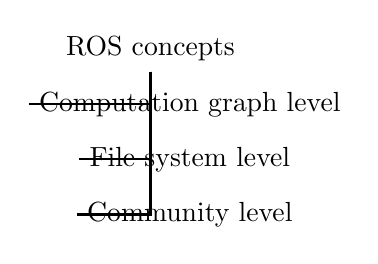
\begin{tikzpicture}[%
thick, grow via three points={one child at (0.5,-0.7) and
    two children at (0.5,-0.7) and (0.5,-1.4)},
edge from parent path={(\tikzparentnode.south) |- (\tikzchildnode.west)}]
\node {ROS concepts}
child { node {Computation graph level}}
child { node {File system level}}	
child { node {Community level}};
\end{tikzpicture}
\end{frame}

\subsection{Computation graph level}

\begin{frame}{Computation graph level}
    \framesubtitle{ROS concepts}
    \begin{itemize}
        \item In an application that uses ROS, the computations are executed by a collection of elements processing data together.
        \item It comprises of executables and connections between them.
    \end{itemize}
\end{frame}

\begin{frame}{Computation graph level}
    \framesubtitle{ROS concepts}
    
    Concepts related to ROS computation graph:
    
    \begin{enumerate}
        \item Nodes
        \item Topics
        \item Messages
        \item Services
        \item Actions
        \item Bags
    \end{enumerate}
\end{frame}

\begin{frame}{Computation graph level}
    \framesubtitle{ROS concepts}
    {\huge Nodes:}
    % \vspace{1cm}
    \begin{itemize}
        \item It is the basic functional block of code that performs a function eg publish to robot velocity(cmdvel), receive laser scan data(scan)
        \item A ROS node is a process that exchanges data with other processes through ROS network.
        \item It may be a python script, a C++ written process, or even a MATLAB script.
        \item The advantage of ROS is that you can write your nodes in different languages and can still make them work together 
       \item They can be run on single or multiple computers and are connected together in a peer-to-peer network.
    \end{itemize}
\end{frame}

       
     \begin{frame}[plain]{}
         \begin{textblock}{5}(5,10)
             \includegraphics[width=0.5\linewidth]{figures/platform.png}
         \end{textblock}
         \begin{textblock}{5}(4,5.2)
             \includegraphics[width=0.7\linewidth]{figures/robot_arm.png}
         \end{textblock}
         \begin{textblock}{5}(5,1.5)
             \includegraphics[width=0.6\linewidth]{figures/kinect.png}
         \end{textblock} 
         \begin{textblock}{5}(9.5,8)
             \includegraphics[width=1.2\linewidth]{figures/pick_and_place.png}
         \end{textblock}           
         \begin{textblock}{5}(0.5,5)
             \includegraphics[width=0.6\linewidth]{figures/nav_comic.png}
         \end{textblock}                      
         \begin{textblock}{5}(9.5,2)
             \includegraphics[width=1.0\linewidth]{figures/object_recognition.jpg}
         \end{textblock} 
         
         \begin{textblock}{5}(0.5,10)
        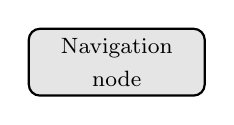
\begin{tikzpicture}
        \node [rectangle,draw,thick,text width=2.0cm,minimum height=0.7cm,
        text centered,rounded corners, fill=black!10] {\footnotesize Navigation node};
        \end{tikzpicture}
         \end{textblock} 

         \begin{textblock}{5}(5.1,3)
             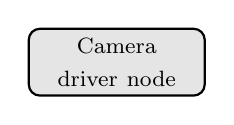
\begin{tikzpicture}
             \node [rectangle,draw,thick,text width=2.0cm,minimum height=0.7cm,
             text centered,rounded corners, fill=black!10] {\footnotesize Camera driver node};
             \end{tikzpicture}
            \end{textblock}
             
         \begin{textblock}{5}(6.5,7)
             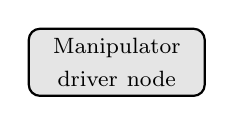
\begin{tikzpicture}
             \node [rectangle,draw,thick,text width=2.0cm,minimum height=0.7cm,
             text centered,rounded corners, fill=black!10] {\footnotesize Manipulator driver node};
             \end{tikzpicture}
            \end{textblock}  

         \begin{textblock}{5}(6.5,11)
             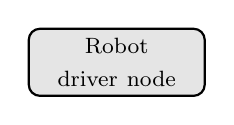
\begin{tikzpicture}
             \node [rectangle,draw,thick,text width=2.0cm,minimum height=0.7cm,
             text centered,rounded corners, fill=black!10] {\footnotesize Robot driver node};
             \end{tikzpicture}
         \end{textblock} 

         \begin{textblock}{5}(12,4)
             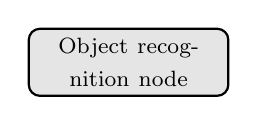
\begin{tikzpicture}
             \node [rectangle,draw,thick,text width=2.3cm,minimum height=0.7cm,
             text centered,rounded corners, fill=black!10] {\footnotesize Object recognition node};
             \end{tikzpicture}
           \end{textblock} 

         \begin{textblock}{5}(12.5,13.5)
             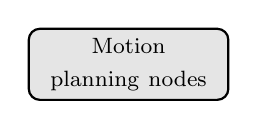
\begin{tikzpicture}
             \node [rectangle,draw,thick,text width=2.3cm,minimum height=0.7cm,
             text centered,rounded corners, fill=black!10] {\footnotesize Motion planning nodes};
             \end{tikzpicture}
            \end{textblock}                                                                     
     \end{frame}                            

\begin{frame}{Computation graph level}
    \framesubtitle{ROS concepts}
    {\huge Topics and messages:}
    \vspace{1cm}
    \begin{itemize}
        \item Nodes send data by publishing messages on a named topic.
        
        \item Nodes receive data by subscribing to a topic.
        
        \item Multiple nodes can publish/subscribe to the same topic.

    \end{itemize}
\end{frame}

\begin{frame}{Computation graph level}
    \framesubtitle{ROS concepts}
    {\huge Topics and messages:}
    \vspace{1cm}
    \begin{itemize}
        \item Publisher node publishes the messages on a topic at a chosen frequency.
        
        \item This \textbf{publish/subscribe} communication paradigm is a many-to-many one-way transport mechanism of data.
        
        \item The publishing node and subscribing node are not aware of each other's existence. 
        
        \item Topic have a defined type eg: topic cmd\_vel has a type of  \textbackslash geometry\_msgs\textbackslash Twist
    \end{itemize}\end{frame}

\setbeamercolor{background canvas}{bg=black}
\begin{frame}[plain]{}  
    \centering
     {\huge \textcolor{white}{Example \\ (TurtleSim)} }
\end{frame}

\setbeamercolor{background canvas}{bg=white}

\begin{frame}{Computation graph level}
    \framesubtitle{ROS concepts}
    {\huge Services:}
    \vspace{0.2cm}
    \begin{itemize}
        \item In many scenarios a publish/subscribe model is not enough, it’s a one-way
        communication.
        
        \item Example scenario: plan a path service.

        \item ROS Services provide an additional way of communication between nodes, a  \textbf{call-and-response} model.
    \end{itemize}  
\end{frame}

\begin{frame}{Computation graph level}
    \framesubtitle{ROS concepts}
    {\huge Services:}
    \vspace{0.2cm}
    \begin{itemize}
        \item It happens between two nodes, the service \textbf{server} node, and the service \textbf{client} node.
        
        \item A Client node calls a service with a request, a node serving this service responds, and the communication is over.
        
        \item A client node call can be synchronous or asynchronous.
        
        \item it is a one-to-one, one-to-many, two-way, one-time communication.
        
    \end{itemize}  
\end{frame}

     
\setbeamercolor{background canvas}{bg=black}
\begin{frame}[plain]{}  
    \centering
    {\huge \textcolor{white}{Example \\ (TurtleSim again)} }
   \end{frame}
\setbeamercolor{background canvas}{bg=white}     
     
        
\begin{frame}{Computation graph level}
    \framesubtitle{ROS concepts}
    {\huge Actions:}
    \vspace{0.2cm}
    \begin{itemize}
        \item ROS services are not suitable for long-term tasks, a client that have sent a service request keeps on waiting for the response from the server. ROS actions solves this.
        
        \item ROS actions can be canceled at any time, and also provides a steady feedback.
        
        \item In ROS actions, client calls are asynchronous.

    \end{itemize}  
\end{frame}


\begin{frame}{Computation graph level}
    \framesubtitle{ROS concepts}
    {\huge Actions:}
    \vspace{0.2cm}
    \begin{itemize}        
        \item Action client can  request for feedback which the action server provides during execution. 
        \item The action nodes can perform other processes depending on this feedback
        eg: Send a goal to robot to move from point A to B but closer the robot gets to point B the robot can slow down 
        \item Once the server finishes executing the task, it sends a result message to the client.
    \end{itemize}  
\end{frame}


\begin{frame}{Computation graph level}
    \framesubtitle{ROS concepts}
    {\huge Bags:}
    \vspace{0.2cm}
    \begin{itemize}
        \item ROS bag is a mechanism for recording data for later playback.
        \item You can record a complete session, with all the topics and messages
        being exchanged along with their time stamping.
        
        \item This is very useful for finding problems in the robot
    \end{itemize}  
\end{frame}

\setbeamercolor{background canvas}{bg=black}
\begin{frame}[plain]{}  
    \centering
    {\huge \textcolor{white}{Example \\ (TurtleSim one last time)} }
   \end{frame}
\setbeamercolor{background canvas}{bg=white}

\begin{frame}{ROS1 and ROS2 differences}
    \framesubtitle{ROS concepts}
    \begin{itemize}
        \item No more \bold{ROS Master}
        \item DDS as middleware
        \item One base library - \textbf{rcl}
        \item Structure of nodes
        \item Components
        \item Lifecycled nodes
        \item No global parameters
        \item QoS - Quality of Service
    \end{itemize}
\end{frame}

\begin{frame}{ROS2 node lifecyle}
    \framesubtitle{ROS2 concepts}
      \centering
    \includegraphics[width=1
    \linewidth]{figures/ROS2_lifecycle.png}
    \tiny{Source: Geoffrey Biggs, Tully Foote, Managed nodes,ROS2 design.}
\end{frame}

\begin{frame}{DDS}
  \framesubtitle{ROS2 concepts}
  \textit{"Data Distribution Service is a middleware protocol and API standard for data-centric connectivity. It is Pub/Sub technology for real-time, dependable and high performance data exchanges."}
  
  \begin{center}
    \textit{DDS is Pub/Sub on Steroids}
  \end{center}
  
  key challenges addressed by DDS:
    \begin{itemize}
        \item \textbf{Real-time:} the delivery of the appropriate information at the appropriate location and time on a continuous basis.
        \item \textbf{Dependable:} assuring reliability, safety, and integrity despite software and hardware failures.
        \item \textbf{High-Performance:} allowing for the rapid distribution of huge amounts of data.

    \end{itemize}

\tiny{Source: The DDS Tutorial by Angelo Corsaro. }
\end{frame}

\subsection{File system level}

\begin{frame}{File system level}
  \framesubtitle{ROS concepts}
    
 \centering
 \scalebox{0.9}{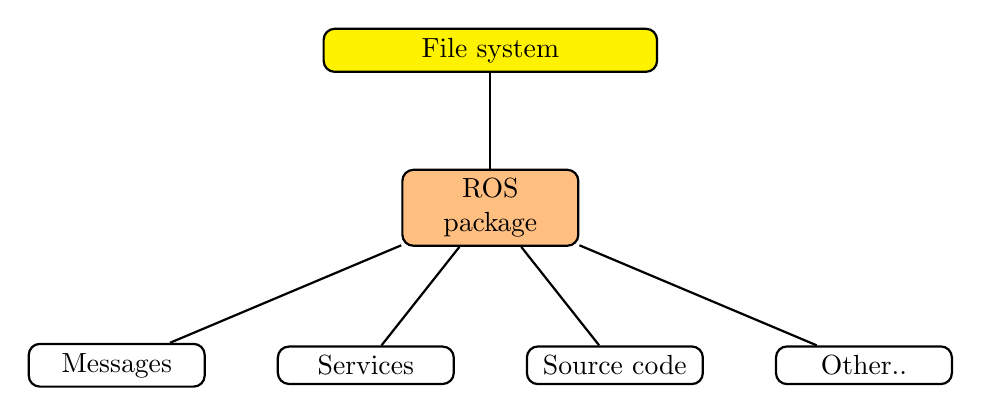
\begin{tikzpicture}[sibling distance=9em, level distance = 2.0cm, thick,
     every node/.style = {shape=rectangle, rounded corners,
         draw, align=center}]]
        \node [text width=4cm, fill = yellow]{File system}
         child { node [text width=2cm, fill = orange!50]{ROS package} 
        child { node [text width=2cm]{Messages} }
        child { node [text width=2cm]{Services} }
        child { node [text width=2cm]{Source code} }
        child { node [text width=2cm]{Other..} }
        };
        \end{tikzpicture}}
\end{frame}


\begin{frame}{File system level}
    \framesubtitle{ROS concepts}
    
    \centering
    \scalebox{0.9}{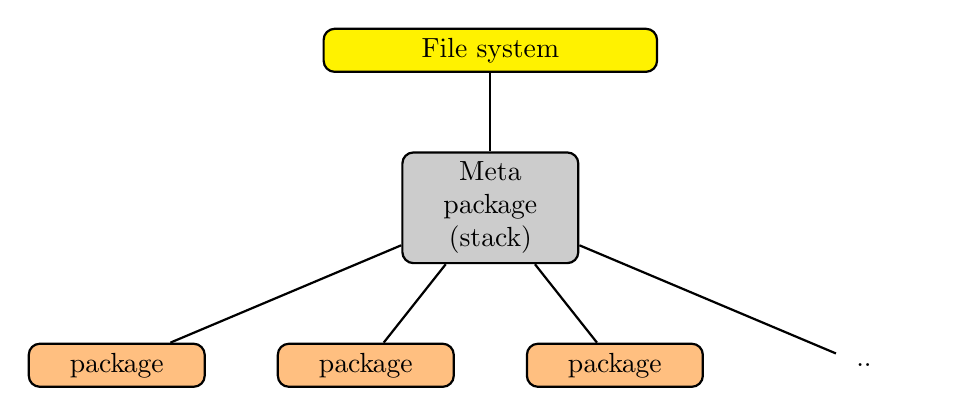
\begin{tikzpicture}[sibling distance=9em, level distance = 2.0cm, thick,
        every node/.style = {shape=rectangle, rounded corners,
            draw, align=center}]]
        \node [text width=4cm, fill = yellow]{File system}
        child { node [text width=2cm, fill = black!20]{Meta package \\ (stack)} 
            child { node [text width=2cm, fill = orange!50]{package} }
            child { node [text width=2cm, fill = orange!50]{package} }
            child { node [text width=2cm, fill = orange!50]{package} }
            child { node [text width=2cm, fill = none, draw = none]{..} }
        };
        \end{tikzpicture}}
% Metapackages are specialized Packages in ROS2 (and catkin). They do not install files (other than their package.xml manifest) and they do not contain any tests, code, files, or other items usually found in packages. A metapackage is used in a similar fashion as virtual packages are used in the debian packaging world. A metapackage simply references one or more related packages which are loosely grouped together.


\end{frame}


\begin{frame}{File system level}
    \framesubtitle{ROS concepts}
Inside a ROS package:

\vspace{0.5cm}
\centering
\includegraphics[width=.9\linewidth]{figures/example_package.png}
\end{frame}
    


\subsection{Community level}
\begin{frame}{Community level}
    \framesubtitle{ROS concepts}
    
    Concepts related to ROS2 development process and it's community:
    
    \begin{enumerate}
        \item The ROS Wiki.
        \item Repositories.
        \item Mailing Lists.
        \item ROS Answers.
        \item ROS Distributions.
    \end{enumerate}
\end{frame}

\section{References}
\begin{frame}{References}

    \begin{enumerate}
        \item \href{http://wiki.ros.org/ROS/Introduction}{ROS Wiki}.
        \item \href{http://design.ros2.org/articles/why_ros2.html}{ROS2 Wiki, on the drawbacks of ROS}.
        \item \href{https://docs.ros.org/en/rolling/Tutorials/Beginner-CLI-Tools/Understanding-ROS2-Services/Understanding-ROS2-Services.html}{Overview on ROS services.}
        
         \item \href{https://docs.ros.org/en/rolling/Tutorials/Beginner-CLI-Tools/Understanding-ROS2-Actions/Understanding-ROS2-Actions.html}{Overview on ROS actions.}   
             
        \item \href{https://wiki.ros.org/Events/CoTeSys-ROS-School?action=AttachFile&do=get&target=ros_tutorial.pdf}{ROS introduction slides by Rada}.
        
        \item ROS Client Libraries     \color{blue}{\href{http://wiki.ros.org/Client\%20Libraries}{ROS1}},
        \color{blue}{\href{https://docs.ros.org/en/rolling/Concepts/About-ROS-2-Client-Libraries.html}{ROS2}}.
        \color{black}
        \item Previous material of the foundation\_course. 
    \end{enumerate}
\end{frame}



\setbeamercolor{background canvas}{bg=black}
\begin{frame}[plain]{}  
    \centering
    {\huge \textcolor{white}{Thank you}}
    
    \vspace{0.5cm}
    
    {\huge \textcolor{white}{Any questions?}}
\end{frame}
\setbeamercolor{background canvas}{bg=white}


\end{document}
